%%%%%%%%%%%%%%%%%%%%%%%%%%%%%%%%%%%%%%%%%%%%%%%%%%%%%%%%%%%%%%%%%
\chapter{KULLANILABİLECEK TEKNOLOJİLER}\label{CH2}
%%%%%%%%%%%%%%%%%%%%%%%%%%%%%%%%%%%%%%%%%%%%%%%%%%%%%%%%%%%%%%%%%
\section{PYTHON GÖRÜNTÜ İŞLEME KÜTÜPHANELERİ}
\cite{artifical}
Görüntü İşleme alanında programlama yapmak için günümüzde birçok farklı alternatif bulunmaktadır. En temel düzeyde iki sınıfa ayırmak gerekirse, bunlardan biri yapay zeka destekli ( YOLO vb.) görüntü işleme çalışmaları, diğeri de belirli kütüphane ve frameworkleri kullanarak herhangi bir machine learning ya da deep learning tekniği kullanmaksızın kendi  algoritmalarımızı geliştirmektir.
Python zengin kütüphane ve framework seçenekleri ile adından söz ettirdiği gibi bu alanda da birçok alternatif bulundurmakta. Python Görüntü İşleme Kütüphaneleri arasından başı OpenCv çeker, bununla beraber SimpleCV gibi de frameworkler bulundurmaktadır. OpenCv ‘nin yanı sıra Yapay Zeka ve Makine öğrenmesi üzerine büyük avantajları bulunan Python’da Deep Learning tabanlı kendi Image Processing algoritmalarınızı da geliştirebilirsiniz.

\subsection{Numpy Kütüphanesi}
Numpy, bilimsel hesaplama işlemleri,çok boyutlu diziler, çeşitli türetilmiş nesneler dahil olmak üzere diziler üzerinde hızlı işlemler yapılabilmesi için kullanılan önemli kütüphanelerden birisidir.
Numpy, veri tipi olarak n boyutlu dizinin tanımlanmasını sağlar ve diziler üzerinde yeniden boyutlandırma, indeksleme gibi temel işlevlerin gerçekleştirilmesinde kullanılır.\\
\subsection{Matplotlib Kütüphanesi}
Matplotlib, çeşitli basılı formatlarda ve interaktif ortamlarda yüksek kalitede görüntüler üretebilen iki boyutlu çizim kütüphanesidir. Matplotlib, Python komut dosyalarında, Python ve IPython kabuklarında, Jupyter dizüstü bilgisayarında, web uygulama sunucularında ve kullanıcı grafik arabirim araçlarında sıklıkla kullanılmaktadır. \\
\subsection{PIL(Python Imaging Library)}
PIL kütüphanesi basit noktasal işlemler, bir dizi yerleşik konvolüsyon çekirdekleri ile filtreleme ve renk alanı dönüşümleri gibi temel görüntü işlevlerini gerçekleştirmek için kullanılan bir kütüphanedir. Python programlama dilinde bu kütüphane kullanılarak görüntü dosyaları üzerinde değiştirme ve dönüştürme işlemleri gerçekleştirilebilmektedir. \\
\subsection{OpenCV Kütüphanesi}
OpenCV, bilgisayarlı görü uygulamaları ve ticari ürünlerde makine öğrenme algısını hızlandırmak için hazırlanmış bir kütüphanedir. OpenCV, 1999 yılında Intel'de Gary Bradski tarafından dünyadaki bilgisayar görüsünün araştırılması ile ticari uygulamaların hızlandırılması amacıyla grafiksel olarak daha güçlü bilgisayarların oluşturulması için tasarlanmıştır.Açık kaynak kodlu ve platformdan bağımsız bir kütüphanedir. \\

\section{GEOMETRİK DÖNÜŞÜMLER}
Görüntü işleme sırasında sıklıkla geometrik görüntü dönüşümlerine ihtiyaç duyulmaktadır. Geometrik dönüşümler, pikseller üzerinde işlemler yaparak görüntü döndüren,daraltan veya büyüten fonksiyonlardır.
\newpage
 \subsubsection{Bilineer İnterpolasyon}
Görüntü üzerinde eski piksel değeribaz alınarak farklı bir noktadaki yeniğ pikselin olası değerinin hesaplanması yöntemidir. Başka bir ifadeyle örnekleme olarak ifade edilir. 
\subsubsection{Affin Dönüşümü}
•\textbf{üç temel işlem}:Görüntüler üzerinde koordinaqt dönüşümlerine dayalı üç temel işlem olan ölçekleme, döndürme ve öteleme işlemleridir.
•\textbf{affin dönüşüm bağıntısı}:Birbirine paralel olmayan (dik veya eğik) iki düzlemden biri, diğeri üzerine izdüşümlendirilirse görüntü ve esas şekil arasında bir affin dönüşüm bağıntısı elde edilir.
\subsubsection{Öteleme}
Görüntüyü öteleme işlemi, piksellerin değerleri değişmeden koordinat sistemindeki konumunun değiştirilmesi olarak tanımlanmaktadır.
\subsubsection{Döndürme}
Görüntünün döndürülmesi, görüntüdeki piksellerin belirli bir açıda döndürülmesi ile piksel konumlarının değiştirilmesi işlemidir.
\subsubsection{Aynalama}
Görüntüyü yansıtma işlemi, belirli bir nokta ya da eksen etrafında orjinal görüntüdeki piksellerin yansıtılarak yeni konumlarına yerleştirilmesi işlemidir.
\subsubsection{Ölçeklendirme}
Görüntüyü ölçeklendirme işlemleri, görüntüler üzerinde belirli bir alanda ya da görüntünün tamamında görüntünün büyütülmesi veya küçültülmesi için kullanılmaktadır.
Küçültme-Büyültme
Piksel Değiştirme
Piksel İnterpolasyonu
Eğme-Kaydırma
\section{HİSTOGRAM EŞİTLEME}
\cite{platereg} Histogram eşitleme işlemi bir resim üzerideki piksel değerlerinin arasındaki farkları en aza indirme işlemidir. Bir nevi map fonksiyonu gibi düşünülebilir. Histogram eşitleme işlemi piksel değerlerini sadece kaç adet olduklarını bulmak için kullanırken adet değerlerinin cdf* ile hesaplanmış hallerinden yeni görüntüyü oluşturur.
Bu işlemi gerçekleştirmek için işlem adımları aşağıda verilmiştir;

Her pikselin tekrar sayısını bul(histogram dizisi),
Pikselleri Değerlerine göre sırala,
Bu değerler üzerinden cdf toplam matrisi oluştur,
Her bir cdf değeri için cdf fonksiyonunu işlet,
Gerçek resim üzerindeki piksel değerlerini cdf piksel değerlerine göre değiştir.
\section{RENK UZAYLARI}
\cite{imagep} Renk uzayları, görüntüde oluşan renk içerikleri üç veya dört farklı renk bileşenleriyle birlikte matematiksel model oluşturmaktadır.
\subsection{HSV Renk Uzayı}
\cite{hsv}
HSV, bir silindir şeklinde ifade edilir. Piksel değeri x için, H değeri x’ in açısal konumunu ifade eder, S değeri x’ in silindirin merkezine uzaklığını, V değeri ise x’ in silindir yüzeyine uzaklığını ifade eder.HSV sisteminde H ve S değerlerinin ne olduğuna bakmaksızın eğer V değeri sıfıra eşitse 0 ise ortaya çıkan renk siyah olacaktır.
\subsection{RGB Renk Uzayı}
\cite{rgb}
 RGB renk modelinin temel olarak doğada bulunan tüm renklerin yalnızca üç rengin referansı ile oluşturulabilmesine dayanır. Bu üç renk ise kırmızı, yeşil ve mavidir. Daha anlaşılır bir ifadeyle, RGB renkler ışık bazlı olduklarından dijital ekranlarda renkli görüntü elde etmeyi mümkün kılmaktadır. Bu nedenle eğer dijital ekranlarda görüntülenecek bir tasarımınız varsa, kullandığınız tasarım programında mutlaka RGB renkleri seçmeniz gerekmektedir. Bu sayede daha canlı tasarımlar elde edebilirsiniz.


 \section{GÖRÜNTÜ İŞLEMEDE KULLANILAN TEMEL FİLTRELER}
 \subsection{Ortalama (Mean) Filtreleme Yöntemi}
\cite{filtreleme}Ortalama filtresi, görüntüleri yumuşatmanın basit ve uygulanması kolay bir yöntemidir. Diğer bir deyişle, bir piksel ile diğerleri arasındaki değişim miktarını azaltmaktır. Genellikle görüntülerdeki gürültüyü azaltmakiçin kullanılır.Ortalama filtresi, bir görüntünün her bir piksel değerini komşularının ve kendisinin dahil olduğu ortalama değer ile değiştirmektir. Bu durum, çevresindekileri temsil etmeyen piksel değerlerinin ortadan kalkmasına yol açar. Ortalama filtresi bir konvolüsyon filtresidir. Konvolüsyon filtreleri çekirdek şablon (kernel)temeline dayanır. 
\subsection{Medyan Filtreleme Yöntemi}
Medyan filtresi, normal olarak mean filtresi gibi bir resimdeki gürültüyü azaltmak için kullanılır. Ancak resim üzerindeki detayların kaybolmaması noktasında mean filtresinden çok daha iyi sonuç verir. Medyan filtre de mean filtresi gibi her pikselin değerini hesaplamak için yakınındaki komşularına bakar. Medyan filtresinde piksel değeri komşu piksel değerlerinin ortalaması ile değiştirmek yerine (mean filtresi), komşu pikselleri sıralayıp sıranın ortasındaki değeri alır. Eğer incelenen bölge (şablonun içerisi) çift sayıda piksel varsa,orta değer olarak, ortada bulunan iki pikselin ortalaması kullanılır.
\subsection{Gaussian Filtreleme Yöntemi}
Gauss yumuşatma operatörü, görüntüleri 'bulanıklaştırmak', ayrıntı ve gürültüyü ortadan kaldırmak için kullanılan 2 boyutlu konvolüsyon (çekirdek matris ile resim üzerindeki piksellerin çarpımı işlemi) operatörüdür. Bu anlamda, ortalama (Mean) filtreye benzer. Ancak Gauss, "çan şeklindeki" grafikle temsil edilebilecek farklı bir çekirdek şablon (matris) kullanır. 
\subsection{Sobel Filtreleme Yöntemi}
Sobel filtre görüntülerdeki objelerin sınırlarını tespit etmek için kullanılan bir filtreleme yöntemidir.Görüntü üzerinde hem yatay hem de dikey olarak kenar belirleme yapılabilmektedir.
\subsection{Laplasian Filtreleme Yöntemi}
Laplacian operatörü, görüntü netleştirme, kenar algılama ve kenar hatlarını belirleme işlemlerinde sıklıkla kullanılmaktadır.
\subsection{Konservatif Filtreleme Yöntemi}
Görüntü üzerindeki gürültüleri azaltmak için kullanılan bir yöntemdir.Gürültü, görüntüdeki ayrıntıların görülme miktarını azaltırken konservatif filtreleme ile bu problem hızlı bir şekilde azaltılarak keskin kenarlar korunmaktadır.
\subsection{Fourier Dönüşüm Filtreleme Yöntemi}
Furier dönüşümünde filtreleme işlemi frekans boyutunda gerçekleşmektedir. Fourier dönüşümü frekans alanındaki görüntüyü ifade ederken, girdi görüntüsü uzaysal alanı ifade etmektedir. Kısacası Fourier bir görüntünün kosinüs ve sinüs bileşenlerini ayırmak için kullanılmaktadır.

\section{EŞİKLEME İŞLEMLERİ}
\cite{segmentation}
Eşikleme genel olarak gri tonlu görüntüden ikili görüntü elde etmek için kullanılan bir filtreleme yöntemidir. Eşikleme işlmeleri statik ve dinamik eşitleme olmak üzere iki kategoriye ayrılır.
\subsection{Statik Eşikleme}
Statik eşiklemede ikili tip, ters ikili tip, sıfır tip, ters swıfır tip ve kırpmaq tip olmak üzere beş kategoriye ayrılır.
\subsection{Dinamik Eşikleme}
Otsu algoritması olarak da bilinir. Görüntüdeki piksellerin kümelenmesini piksel değerlerinin dağılımına göre sağlamaktadır. Görüntüdeki piksel sayılarını hesaplamada kullanılan matematiksel ifadeleri mevcuttur.

 \section{MORFOLOJİ İŞLEMLERİ}
\cite{image_proc} Bazen, görüntünüzü eşledikten sonra, ikili görüntünüzde istenmeyen parazit olur. Morfolojik işlemler bu gürültüyü görüntüden çıkarmaya yardımcı olabilir.
\subsection{Çekirdek}
Çekirdek, başlangıç noktasının ikili görüntünün 1 değerinin her pikselinin üzerine yerleştirildiği basit bir şekildir. OpenCV, çekirdeği NxN matrisiyle sınırlar, burada N tek sayıdır. Çekirdeğin kökeni merkezdir.
\subsection{Erozyon}
Bilgisayarla görmedeki erozyon, topraktaki erozyona benzer. Ön plandaki nesnelerin sınırlarından uzaklaşır. Bu işlem arka plandaki gürültüyü ortadan kaldırabilir.
\subsection{Dilation-Genişleme}
Genleşme erozyonun tam tersidir. Sınırlardan uzaklaşmak yerine onlara katkıda bulunuyor. Bu işlem, daha geniş bir bölgedeki küçük delikleri kaldırabilir.
\subsection{Opening-Açılış}
Açılma erozyon ve ardından genişlemedir. Bu işlem, daha büyük özelliklerin şeklini etkilemeden gürültüyü ortadan kaldırır.
\subsection{Closing-Kapanış}
Kapatma genişlemedir ve ardından erozyon meydana gelir. Bu işlem, daha büyük unsurların şeklini etkilemeden küçük delikleri veya kırılmaları giderir.

\section{PLAKA TANIMA ADIMLARI}
\cite{plate}Plaka tanıma işlemi yapmak için yedi temel algoritma vardır. Bu algoritmalar ile plaka bulma işlemi yapılmaktadır. Bu algoritmaların hassasiyeti plaka bulma işleminde çok fazla etkilemektedir.\cite{plakatanımlama} Plaka tanıma işlemlerinde kullanılan algoritmalar şunlardır;
\begin{itemize}
\item Plaka yerinin tespiti
\item Plakanın sonraki algoritmalara uygun bir biçimde yeniden konumlandırılması ve boyutlandırılması
\item Zıtlık ve parlaklık gibi görüntü özelliklerininnormalizasyonu
\item Karakter ayırma ile görüntü üzerinden karakterlerinçıkarılması
\item Optik karakter tanıma
\item Ülkeye özgü kelime dizimi ve kontrol işlemi
\item Daha güvenilir bir sonuç elde etmek için tanımlanan değerin birden fazla görüntüde ortalamasının alınması
\end{itemize}
\subsection{Görüntü Üzerinden Plakanın Ayrıştırılması}
\cite{platereg} Görüntü üzerindeki plaka kısmının doğru bir şekilde ayrılması oldukça önemlidir. Bu adımda yapılacak bir yanlış sistemin tamamını etkilemektedir. Plakanın görüntü üzerinden ayrılmasında belirli koşullar vardır. Sistem tasarlanırken hava koşulları, parlaklık gibi kriterler önemlidir. Tüm şartlarda üst seviyede çalışabilecek sistem tasarlanması için burada yapılacak işlemler önemlidir. Sistem günün her saatinde çalışması gerektiği için alınan görüntler farklı kontrast değerlerine sahip olacaklardır. \\
\cite{video_proc} İşlemler sırasıyla ilk olarak alınan görüntünün griye çevrilir. Griye çevrilen resim üzerinde gürültü temizleme işlemi yapılır. Görüntü üzerinde histogram eşitleme işleme işlemi yapılır. Morfolojik işlem uygulanır. Histogram eşitleme yapılan görüntüden, morfolojik işlem yapılmış işlem piksel piksel çıkartılır. Görüntü eşikleme işlemi yapılır. Canny edge uygulanır. Genişletme işlemi yapılır. Kontur işlemi gerçekleştirilir.Son olarak plaka bölgesi maskeleme yapılarak görüntü üzerinden ayrıştırılır.
\subsection{Görüntü Ön İşleme}
\cite{digital}
 
\end{itemize}
\subsubsection{Rgb’den gri seviyeli görüntüye dönüştürme işlemi} Resim işleme alındığı zaman ilk olarak RGB uzayındadır. Görüntü üzerinde işlemlerimizi daha basit ve daha kolay bir şekilde plaka yerini tespit etmek için görüntü Rgb’den gri seviyeli görüntüye dönüştürme işlemi yapılır. Rgb modeli üç ana renk olan kırmızı, yeşil ve mavi renklerini içermektedir. Gri seviyeli bir resme sahip olmak için kırmızı kanalın %30 ‘u, yeşil kanalın %59’ u ve mavi kanalın %11’lik kısmı alınmaktadır. Renkli bir resim ile gri seviye bir resim arasındaki fark, renkli resmin bir pikselinde üç farklı renk vardır.Gri seviyede sadece tek bir değer vardır. Bu üç farklı 0 ile 255 arasında değişen değerleri tek bir 0 ile 255 arasında değişen değer haline getirmek gerekir.
\begin{figure}
    \centering
    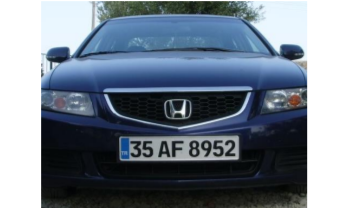
\includegraphics{rgb.PNG}
    \caption{RGB renk uzayında plaka görünümü}
    \label{fig:my_label}
\end{figure}
\subsubsection{Gri seviyeli resim üzerinde gürültü temizleme}
\cite{shape} Gürültü temizlemek için ortalama alma , medyan ortalama, bileteral filtreleme gibi çeşitli algoritmalar bulunmaktadır. Bu algoritmalar içerisinde görüntü üzerinde en güçlü gürültüyü azaltan filtre bileteral filtreleme işlemdir. Bileteral filtreleme işlemi kenaraları keskin bir hale getirerek gürültünün giderilmesinde oldukça etkilidir. Fakat diğer filtrelere göre biraz daha yavaştır. Plaka tanıma sistemde plaka kenarlarının net bir biçimde ortaya çıkmasını sağlamak ve kaybolan kenarları netleştirmek ortaya çıkarmak için bileteral filtre 
kullanılmıştır.
\begin{figure}
    \centering
    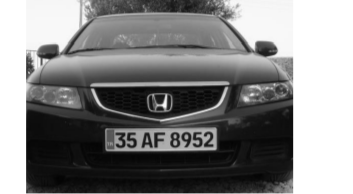
\includegraphics{gri seviye plaka.PNG}
    \caption{Gri seviyeye dönüştürülmüş plaka}
    \label{fig:my_label}
\end{figure}
\subsubsection{Histogram Eşitleme İşlemi}
\cite{platereg}
Plaka tanıma sisteminde plakalar tanınırken ortam, ışık, renk gibi değişiklikler olabilir. Sistemin bunun gibi çevresel etkenlerden etkilenmesini azaltmak için görüntü üzerinde histogram eşitleme işlemi yapılmaktadır. Bir görüntünün histogramı, o görüntü hakkında önemli bilgiler verir. Karanlık bir resim grafiğinin düşük gri seviye bölgesine yığılmaktadır. Parlak bir görüntüde ise büyük gri seviyesine yığılmaktadır. Alınan görüntü üzerinde histogram eşitleme işlemi gerçekleştirilerek görünütüyü iyileştirme işlemi gerçekleştirilir.

\begin{figure}
    \centering
    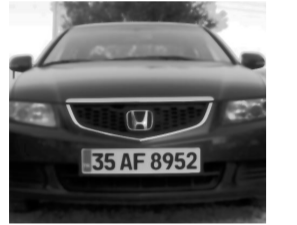
\includegraphics{histogram filtre.PNG}
    \caption{Histogram eşitleme işleminden geçmiş plaka görüntüsü}
    \label{fig:my_label}
\end{figure}
\subsubsection{Morfolojik İşleme İşlemi}
\cite{detection}
Mofolojik işlem ile görüntü üzerinde aşındırma ve genişletme işlemleri yapılabimektedir. Bu filtre ile görüntü üzerindeki gürültünün giderilmesi ile daha doğru sonuçlar elde edilmektedir. Bu filtre ile görüntü üzerinde açma işlemi gerçekleştirilmiştir. Aşındırma işlemi ile küçük paralar yok edilerek görüntü tekrar genişletilmiştir.
\begin{figure}
    \centering
    \includegraphics{morfolojik işlem.PNG}
    \caption{Morfolojik işlem sonrası meydana gelen plaka resmi}
    \label{fig:my_label}
\end{figure}
\subsubsection{Pixel Çıkarma İşlemi}
\cite{vision} Pixel çıkarma veya görüntü çıkarma işlemi bir görüntünün veya piksellerinin sayısal değerlerinin başka bir görüntüden çıkarılması ile ortaya çıkan bir işlemdir. Bir görüntü üzerinde düzensiz olan bölgeleri dengelemek ve iki resim arasındaki değişiklikleri saptamak için kullanılmaktadır. Plaka tanıma sisteminde amacımız plaka bölgesinin net bir şekilde ortaya konularak , diğer bölgelerin görünürlüğünü azaltmaktır. Histogram eşitleme yapılmış bir resim üzerinden morfolojik işlem yapılan resim çıkartılarak bu adım gerçekleştirilmektedir.
\begin{figure}
    \centering
    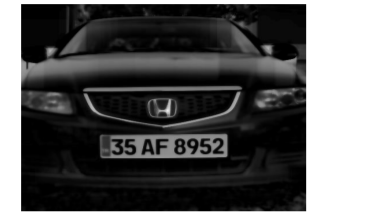
\includegraphics{pixel çıkarma işlemi.PNG}
    \caption{Pixel çıkarma işlemi uygulandıktan sonra elde edilen plaka görüntüsü}
    \label{fig:my_label}
\end{figure}
\subsubsection{Görüntü Eşikleme İşlemi}
\cite{shape}
Görüntü üzerinde belirli bir eşik değeri altında kalan kısımları 0 üstünde kalan kısımları ise 1 yapmak süretiyle ikili bir görüntü oluşturma işlemi yapılmasıdır. Bu sistemde ortam şartları sürekli değişmektedir. Eşik değeri her görüntü için farklı olmaktadır. Elle eşik değeri belirlemek gömülü sistem üzerinde çalışan uygulamalar için mümkün olmayacağı için görüntü üzerinde eşik değeri belirli algoritmalar sayesinde hesaplanmaktadır. Eşik değeri belirlemede Nobuyuki Otsu 1975 yılında yayınladığı yazıda Otsu modelini tanıtmıştır. Otsu modelinde varyans denilen bir değer hesaplanır ve değerin en düşük olduğu indeks döndürülmektedir. Görüntü üzerinde eşik değerini hesaplamak için Otsu modelinden yararlanılmaktadır.Pixel çıkarma işlemi uygulanmış ve plaka bölgesi net bir biçimde ortaya çıkmış resimde görüntü eşikleme işlemi yapılarak plaka bölgesinin daha net olarak ortaya çıkması sağlanmıştır.
\begin{figure}
    \centering
    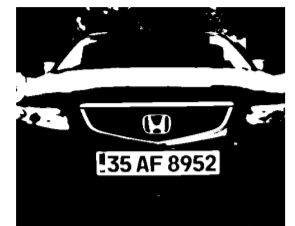
\includegraphics{görüntü eşikleme.PNG}
    \caption{Görüntü eşikleme işlemi yapılmış olan plaka}
    \label{fig:my_label}
\end{figure}
\subsubsection{Kenar algılama işlemi}
\cite{skeletonization} Canny edge algoritması kenar algılalama için kullanılan bir algoritmadır.Görüntü üzerindeki plaka tanıma işlemi yapmak için kenarlar belirlenmesi gerekmektedir. Canny edge çeşitli görme sistemlerinde kenar algılama uygulaması olarak kullanılmış ve başarılı bir şekilde görüntü üzerindeki kenarları ortaya çıkarmayı başarmıştır. Canny algoritması süreci adımlar halindedir. Canny kenar algılama algoritması düşük hata oranı ile kenarları bulması için gürültüyü gidermek için ilk olarak bileteral filtresi uygulanmıştır. Bileteral filtresi yerine gauss filtreside uygulanabilir. Bileteral uygulayarak canny edge ile kenar bulma işlemi daha başarılı bi şekilde gerçekleşecektir. Histogram eşitleme işlemi yapılır. Görüntü eşikleme işlemi yapılır. Canny adımları yapılan görüntüde kenarlar ortaya çıkarılmaya çalışılmıştır.
\begin{figure}
    \centering
    \includegraphics{kenar belirginleştirme.PNG}
    \caption{Kenarları belirgin hale getiren plaka görüntüsü}
    \label{fig:my_label}
\end{figure}
\subsubsection{Genişletme İşlemi}
Canny edge uygulanan görüntü üzerine uygulanmıştır. Canny edge uygulanarak kenarları yüksek bir oranda algılama işlemi gerçekleştirilmiştir. Kenarları genişletmek için daha belirgin hale getirmek için dilate işlemi yapılır. Genişletme işlemi yapmak için bir çekirdek matris oluşturulur. Bu uygulamada 3x3 lük birler matrisi ile işlemleri gerekleştirilir. Bir merkezi nokta seçilir oradan başlayarak görüntünün tüm pikselleri üzerinde belirlediğimiz iterasyon sayısı kadar bu işlem gerçekleştirilir. Bu sayade görüntüntü üzerinde darbeler ve noktalar bulunur. Maksimum pixel değerini hesaplar ve görüntü üzerinde bulduğu pikseli maksimum pikselle değiştirir. Pikselleri maksimum değerl ile değiştirmek parlak olan bölgelerin genişlemesini sağlar.
\begin{figure}
    \centering
    \includegraphics{genişletme.PNG}
    \caption{Genişletme işlemi yapıldıktan sonra ortaya çıkanyeni görüntü}
    \label{fig:my_label}
\end{figure}
\subsubsection{Görüntü üzerine kontur uygulanması}
Genişletme işlemi ile kenarları belirgin bir görüntü elde edilir. Elde edilen görüntü üzerinde gereken işlem kontur uygulayarak aranan plaka bölgesini işaretlemektir.Konturlar, aynı renk veya yoğunluğa sahip olan tüm kesintisiz noktaları (sınır boyunca) birleştiren bir eğri olarak basitçe açıklanabilir. Konturlar, şekil analizi ve nesne algılama ve tanıma için yararlı bir araçtır.Kontur yapmadan önce konturun doğru sonuç vermesi için canny edge ve genişletme işlemi uygulanır. Sınır noktalarınızın olması koşuluyla herhangi bir şekli çizmek için de kullanılabilir. Buna göre istediğimiz alanları bulmak için bulması gereken parametreler önceden belirlenmiştir. Buna göre görüntü üzerindeki dikdörtgen bölgeyi arama işlemi yapılmıştır. Aradığı bölgeleri bulduktan sonra dört köşesini işaretleteme işlemi yapılmıştır. Bulunan bu bölgeleri çerçeve içerisine alınmışıtr.Görüntü üzerinde uygulanan kontur sonrasında plaka bölgesinin bulunması işlemi gerçekleştirilmiştir. Bulunan plaka bölgesi çerçeve içersine alınmıştır.
\begin{figure}
    \centering
    \includegraphics{kontur işlemi.PNG}
    \caption{Kontur işlemi plaka görüntüsü}
    \label{fig:my_label}
\end{figure}
\subsubsection{Plaka bölgesinin maskelenmesi}
\cite{plate}
Kontur uygulanan resim ile plaka çerçevesi buldurma işlemi gerçekleştirilmiştir. Görüntü üzerinden plakayı ayrıştırmak için maskeleme işlemi yapılır. Maskeleme yaparak bundan sonraki işlemlerde sadece plaka üzerinde işlemler gerçekleştirilir. 
\begin{figure}
    \centering
    \includegraphics{plaka bölgesi bulma.PNG}
    \caption{Kontur ile plaka bölgesinim bulunması ve etrafının
çerçevelenmesi}
    \label{fig:my_label}
\end{figure}
\section{KARAKTERLERİN PLAKA BÖLGESİNDEN AYRIŞTIRILMASI}
Karakter ayırma işlemi plaka tanıma işlemi yapıldıktan sonra plaka üzerindeki lisans numaralarını yakalamak için kullanılan algoritmadır. Görüntü üzerinde sayıları ve harfleri vurgulayarak görüntüde bulunan diğer nesnelerden ayırmaya çalışır.Karakter tanıma işlemi ile otomatik plaka tanıma, verileri düzenlenebilir hale getirme, aranabilir ve kolayca saklanabilir bilgilere dönüştürür. Görüntüye uygulanan belirlenmiş algoritmalardır. 
\\
\cite{complex}
Plakayı bulmak için gerekli filtreler görüntü üzerinde uygulanması gerekir. Bu adımlar karakterlerin daha net bir biçimde gözükmesini doğruluk oranının artmasını sağlayacaktır. Plaka tanıma işleminde en kritik süreç karakter ayrıştırılması işlemidir. Görüntü üzerinden kesilen plaka bölgesi resim üzerinde düzgün bir biçimde olmayabilir. Karakterlerin tamamı aynı hizada değildir.Karakterlerin aynı hizada olması karakterin ayrıştırılması için önemli bir etkendir. Kaliteli bir biçimde ayrıştırma yapmak için eğim açısı tespit edilir.Aynı açıyla ters yönde döndürerek plaka x ekseni üzerinde paralel hale gelir. Plaka üzerindeki karakterler eğim işlemi sonucunda aynı hizaya gelecektir. Karakterlerin üst ve alt sınırları belirlendikten sonra karakter ayrıştırma işlemi gerçekleştirilir.
\begin{figure}
    \centering
    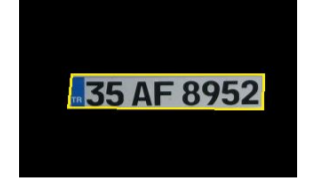
\includegraphics{kırpma.PNG}
    \caption{:Bulunan plaka yerinin fotoğraftan kırpılması işlemi}
    \label{fig:my_label}
\end{figure}
\subsection{Plaka üzerinde eğimin düzeltilmesi}
\cite{detection}
Karakter ayrıştırma işleminin başarılı bir biçimde gerçekleştirmek için x eksenine göre eğim tespiti yapılması gerekmektedir. Eğim bulunan resmin x eksenine paralel bir biçimde gelmesi sağlanmalıdır.Eğim tespiti için karakterlerin x eksenine göre başlangıç ve bitiş noktaları tespit edilir. Y eksenine görede üst sınır ve alt sınır noktaları bulunur. Görüntü üzerinden alınmış karakterlerin yükseklikleri eşittir. Tespit edilen karakterlerin üst sınırları soldan sağa düzenli bir biçimde artma veya azalma gerçekleşiyorsa plaka üzerinde eğim vardır. Bu düzenli artma veya azama değeri tespit edilir, x eksenindeki ve y eksenindeki farkları hesaplanarak eğim açısı bulunur. 
\\
\cite{verification}
Gerekli doğrulamalar yapılmaya başlanır .Eğik plaka üzerinde karakterlerin başlangıç ve bitiş noktaları bulunduktan sonra bu karakterlerin üst ve alt sınırlarının birbirine göre artma veya azalma oranını bulmak gerekir. Karakterlerin üstünde ve altında bulunan plaka çerçevesi, sınırlarının belirlenmesinde edilmesinde bazı durumlarda sorun çıkarmaktadır. Plaka yerini öğrenme yönteminde kullanılan, yan yana olan piksel değerlerinin farkı 20’nin üzerinde olması durumunda, bu pikseller kenar bölgesi kabul edilir. Bu sayede plaka çerçevesi oluşturulduğu için sorun ortadan kalkar.
\begin{figure}
    \centering
    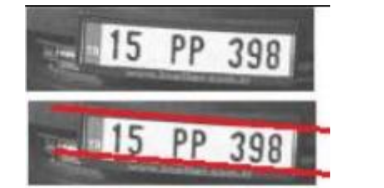
\includegraphics{plaka eğimi.PNG}
    \caption{Plaka üzerinde tespit edilen eğimin örnek görüntüsü}
    \label{fig:my_label}
\end{figure}
\subsection{Plaka üzerindeki karakterleri parçalama işlemi}
Plaka görüntüsünün eğimi düzeltildikten sonra tüm karakterlerin üst ve alt sınırları aynı y düzlemine gelmektedir. Fakat eğimi düzeltilmiş plaka görüntülerinde bile azda olsa x düzlemine göre eğim farklı bulunacağından karakterlerin y sınır eksenleri birebir uymaz, bu durum karakter parçalama için sorun teşkil etmemektedir. Bu aşamadan sonra plaka resminde karakterlerin üst ve alt sınırlarının tespit edilme işlemine gelinmiştir. Yatay düzlemde tarama işlemi yapılarak x ekseninde bulunan siyah piksel noktalarının sayısı bulunur. Görüntünün üst ve alt bölgesinde en az miktarda siyah piksel değerine sahip x ekseni karakterlerin üst ve alt sınırını oluşturmaktadır. Hem hız bakımından hem de bulunan plaka bölgesinde, plaka çerçevesinin oluşturduğu bozulmadan kurtulmak için tüm x eksenini taramak yerine aşağıdaki denklemde gerekli değerler yerine konularak hesaplanır. 
Genişlik: Plaka genişliğinin (1)
X1: x noktası taramanın başlayacağı nokta
X2: x noktası taramanın bitirileceği nokta
X1: (Genişlik / 8 ) * 3
X2: (Genişlik / 8 ) *5;
\begin{figure}
    \centering
    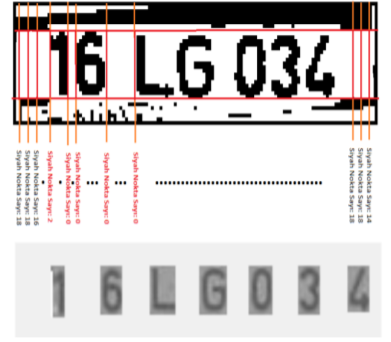
\includegraphics{karakter ayrıştırma.PNG}
    \caption{Plaka üzerinde karakter ayrıştırması yapılması}
    \label{fig:my_label}
\end{figure}
\subsection{Karakterleri tanıma işlemi}
\cite{image_proc} Plaka ayrıştırma sonucunda elde edilen sonuca göre karakterleri tanıma işleminin yapılacağı kısımdır. Plaka karakterlerini tanımlamak için yaygın yöntemler şablon yerleştirme ve yapay sinir ağları yöntemidir. Farklı yazı tipindeki karakterleri tanımlamak için genelde şablon eşleme yöntemi kullanılır. Şablon eşleme yöntemi ile karakter tanıma işlemi yaparken her bir karakterin yükseklik ve genişlllik boyutları sabit biçime getirilmesi gerekir. Karakterler önceden belirlenerek tanıma işlemi gerçekleştirilir.
\begin{figure}
    \centering
    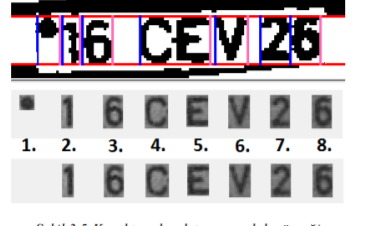
\includegraphics{karakter tanındı.PNG}
    \caption{Karakter tanıma işlemi yapılan plaka görüntüsü}
    \label{fig:my_label}
\end{figure}
\subsection{ Şablon eşleştirme yöntemi}
\cite{imagep} Şablon eşleştirme yöntemi ile karakter tanıma işlemi her bir karakterin piksel değerlerinin önceden programa tanılması ile gerçekleştirilmektedir. Plaka üzerinde bulunan karakterler bu şablondaki karakter ile karşılaştırılması ile yapılır. [14] Karakter tanıma işlemine başlamadan önce şablon çıkarılmalıdır.Şablon eşleştirme yöntemi doğru bir sonuç vermesi için karakterlerin her biri sabit bir boyuta getirilmesi gerekmektedir. Sabit olarak kullanılan karakter boyutu 15x32'dir. Boyutlandırılmış karakterlerin yüksekliği 32 piksel genişliği ise 15 piksel olur. Önceki çalışmalar sonucu en uygun boyut 15x32 olarak belirlenmiştir. Farklı ebatta şablonlar bulunmaktadır. Şablon eşleştirme yöntemi görüntü üzerindeki tüm pikselleri dolaşarak önceden tanıtmış olduğumuz karakterlerin tıtatıp aynısını bulmaya çalışır.
\subsection{Yapay sinir ağları yöntemi}
\cite{yapaysinir}
Yapay sinir ağları karakterleri tanıma işleminde son zamanlarda sıkça kullanılan bir tekniktir. Yapay sinir ağlarında ana amaç insan beyninden yararlanılarak bir olayı öğrenebilmektir.Yapay sinir ağları farklı bir hesaplama yöntemi ile bulunduğu ortama uyum sağlayan ,yetersiz bilgi ile karar verebilen bir sistemdir.[15] Öğrenme işlemi tamamlandığında giriş farklı bir giriş olsa bile doğru bir cevap verebilecek yapıya gelir. İnsan beyninin öğrenme, ilişkilendirme, sınıflandırma, genelleme, ve özellik belirleme gibi konularda uygulanmaktadır. Yapay sinir ağlarında uygulamaya girdiler ve çıktılar verilir. Programa problemin nasıl çözüleceği öğretilir.Yapay sinir ağları üç kısımdan oluşmaktadır. Karakteri belirleme işlemi yaparken karakterin en ve boy oranı vardır. Bundan önce yapılmış ve denenmiş çalışmalara göre bir karakterin eni minumum 5 piksel yüksekliği ise minumum 10 pikseldir. En ve boy altında bulunan her görüntü parazit olarak kabul edilmektedir.
Ayrıştırılan plakar üzerinde karakterleri daha hızlı bir şekilde tanımak için plaka kodlaması üzerinde bulunan harf ve karakterleri daha önceden tanımlamak doğru sonuç alınması açısından fayda sağlayacaktır.
\begin{figure}
    \centering
    \includegraphics{yapay sinir.PNG}
    \caption{Yapay sinir ağları ile karakter tanıma blok diyagramı}
    \label{fig:my_label}
\end{figure}
\section{NEDEN SQLITE VERİTABANI KULLANIYORUM?}
\cite{SQLİTE}
\subsection{Veritabanı Nedir?}
Bilgisayar terminolojisinde, sistematik erişim imkânı olan, yönetilebilir, güncellenebilir, taşınabilir, birbirleri arasında tanımlı ilişkiler bulunabilen bilgiler kümesidir. Bir başka tanımı da, bir bilgisayarda sistematik şekilde saklanmış, programlarca işlenebilecek veri yığınıdır.\\
\subsection{Neden SQLite ?}
Python’da veritabanı işlemleri için kullanabileceğiniz pek çok alternatif bulunur. Ama ben bütün bu alternatifler içinde Sqlite’ı tercih edeceği.m Peki neden Sqlite?

Sqlite’ın öteki sistemlere göre pek çok avantajı bulunur. Gelin isterseniz Sqlite’ın bazı avantajlarına şöyle bir göz gezdirelim :\\
\begin{itemize}
\item Sqlite herhangi bir yazılım veya sunucu kurulumu gerektirmez. Bu sayede, bu modülü kullanabilmek için öncelikle bir sunucu yapılandırmanıza da gerek yoktur. Bazı veritabanlarını kullanabilmek için arka planda bir veritabanı sunucusu çalıştırıyor olmanız gerekir. Sqlite’ta ise böyle bir şey yapmazsınız.
\item Sqlite özgür bir yazılımdır. Bu yazılımın baştan aşağı bütün kodları kamuya açıktır. Dolayısıyla Sqlite kodlarının her zerresini istediğiniz gibi kullanabilir, değişikliğe uğratabilir, satabilir ve ticari olan/olmayan bütün uygulamalarınızda gönül rahatlığıyla kullanabilirsiniz.
\item Her şeyden önce Sqlite Python’un 2.5 sürümlerinden bu yana bu dilin bir parçasıdır. Dolayısıyla eğer kullandığınız Python sürümü 2.5 veya üstü ise Sqlite’ı Python’daki herhangi bir modül gibi içe aktarabilir ve kullanmaya başlayabilirsiniz.
\end{itemize}
\subsection{SQLite Python Kodlarına Nasıl Dahil Edilir?}
Aşağıdaki Python kodu, mevcut bir veritabanına nasıl bağlanılacağını gösterir. Veritabanı yoksa, oluşturulacak ve son olarak bir veritabanı nesnesi döndürülecektir.
\begin{figure}
    \centering
    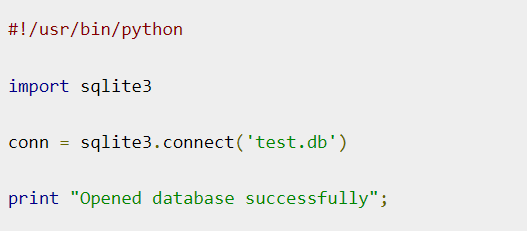
\includegraphics{fig/sql bağlantısı.PNG}
    \caption{Python'a Sqlite bağlantısı kurma kodu}
    \label{fig:my_label}
\end{figure} \\
Daha önce oluşturulan veritabanında bir tablo oluşturmak için aşağıdaki Python programı kullanılacaktır.
\begin{figure}
    \centering
    \includegraphics{fig/tablo oluşturma.PNG}
    \caption{Python ile Sqlite içerisinde bir tablo oluşturma kodu}
    \label{fig:my_label}
\end{figure}
Yukarıdaki program çalıştırıldığında, test.db'nizde COMPANY tablosunu oluşturacaktır. \\
Aşağıdaki Python programı, yukarıdaki örnekte oluşturulan COMPANY tablosunda nasıl kayıt oluşturulacağını gösterir.
\begin{figure}
    \centering
    \includegraphics{fig/insert işlemi.PNG}
    \caption{Python ile Sqlite içerisinde bir tabloya veri kaydı ekleme kodu}
    \label{fig:my_label}
\end{figure}\\
Yukarıdaki program çalıştırıldığında, COMPANY tablosunda verilen kayıtları oluşturacaktır.\\
Aşağıdaki Python programı, yukarıdaki örnekte oluşturulan COMPANY tablosundan kayıtların nasıl getirilip görüntüleneceğini gösterir.
\begin{figure}
    \centering
    \includegraphics{fig/select işlemi.PNG}
    \caption{Python ile Sqlite içerisinde bir tablodan veri kayıtlarını çekme kodu}
    \label{fig:my_label}
\end{figure} \\
Aşağıdaki Python kodu, herhangi bir kaydı güncellemek için UPDATE ifadesinin nasıl kullanılacağını ve ardından COMPANY tablosundan güncellenmiş kayıtları getirip görüntüleyeceğinizi gösterir.
\begin{figure}
    \centering
    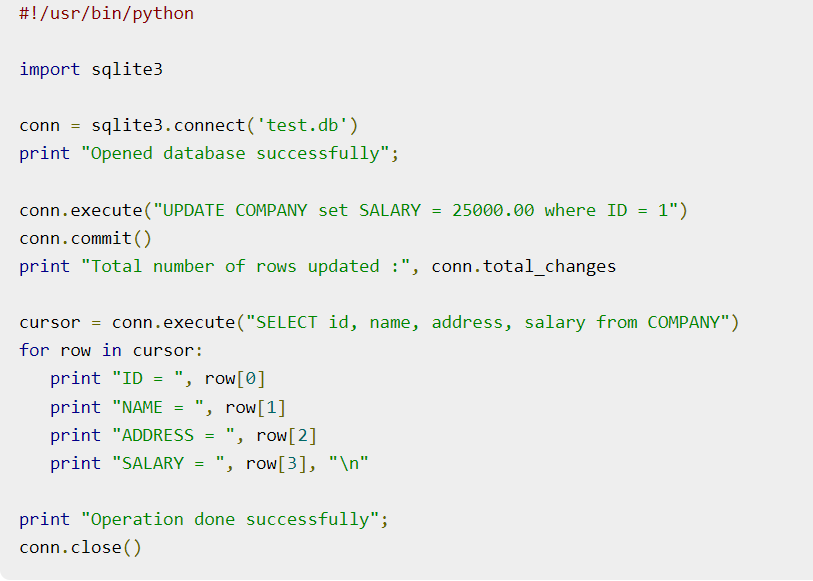
\includegraphics{fig/UPDATE.PNG}
    \caption{Python ile Sqlite içerisinde bir tablodan veri kayıtlarını güncelleme kodu}
    \label{fig:my_label}
\end{figure} \\
Aşağıdaki Python kodu, herhangi bir kaydı silmek için DELETE ifadesinin nasıl kullanılacağını ve ardından COMPANY tablosundan kalan kayıtları alıp görüntüleyeceğinizi gösterir.
\begin{figure}
    \centering
    \includegraphics{fig/delete işlemi.PNG}
    \caption{Python ile Sqlite içerisinde bir tablodan veri kayıtlarını temizleme kodu}
    \label{fig:my_label}
\end{figure} \\
\textbf{Sonuç olarak projemde Python ve Sqlite bağlantısı kurarak , aracın plakasını , otoparka giriş saatini ve aracı bıraktığı konumu veritabanı içerisinde tutuyorum. Daha sonrasında Python içerisinden Sqlite veritabanının barındırdığı verileri çekerek ücret hesaplanması ve aracın konumunun bulunması gibi işlevleri yerine getirebiliyorum. }

\section{PROJE KODLARI VE ÇIKTILARINA AÇIKLAMALI ŞEKİLDE YER VERİLMESİ }
\subsection{Kullanılacak Kütüphanelerin dahil edilmesi}

\begin{figure}
    \centering
    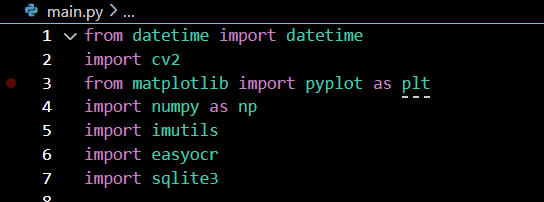
\includegraphics{fig/importlama.PNG}
    \caption{Proje içerisine kütüphanalerin import edilmesi işlemi}
    \label{fig:my_label}
\end{figure} \\

Projenin bu kısmında kullanıcıdan input olarak alınan resim adı içerisinde farklı araç resimleri mevcuttur.Bu araç resimleri görüntü işleme kütüphaneleri yardımıyla tanımlanır ve nihai olarak tanımlanan aracın plakası text olarak geri dönüş yapar.

\textbf{Kod satırlarında açıklamalara yer verilmiştir.}

 \begin{figure}
    \centering
    \includegraphics{resmin işlenmesi.PNG}
    \caption{Kullacıdan alınan resmin işlenme aşamaları}
    \label{fig:my_label}
\end{figure} \\

Şimdi de plakanın tanınmasının diğer aşamalarını inceleyelim. Aşağıdaki kod satırında arac resmi içerisinden plaka kırpılarak çıkarılıyor.
 \begin{figure}
    \centering
    \includegraphics{plakanın kırpılması.PNG}
    \caption{Plakanın araç resmi içeriisnden kırpılması}
    \label{fig:my_label}
\end{figure} \\

Kırpılmış plaka aşamasından sonra plakanın aracnın hangi konumunda olduğunu çevresine bir dikdörtgen çizerek gösteren kod satırına bakalım.
 \begin{figure}
    \centering
    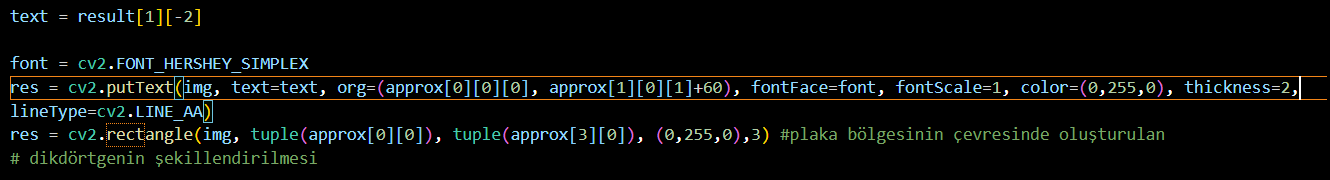
\includegraphics{plakanın çevresine dikdörtgen inşası.PNG}
    \caption{Araç resminde bulunan plaka bölgesinin dikdörtgen içerisinde gösterilmesi}
    \label{fig:my_label}
\end{figure} \\
\cite{pythonsqlbaglantisi}
Projenin bu kısmında SQLİTE bağlantısı gerçekleştiriyoruz ki tanıdığımız plakaların otoparka giriş saatlerini ve aracın konumunu bir veritabanı içerisinde tutabilelim. Böylelikle araç otoparktan çıkarken ne kadar otopark ücreti ödemesi gerektiğini bulabilir ve aracın otopark içerisindeki konumuna erişebiliriz.

 \begin{figure}
    \centering
    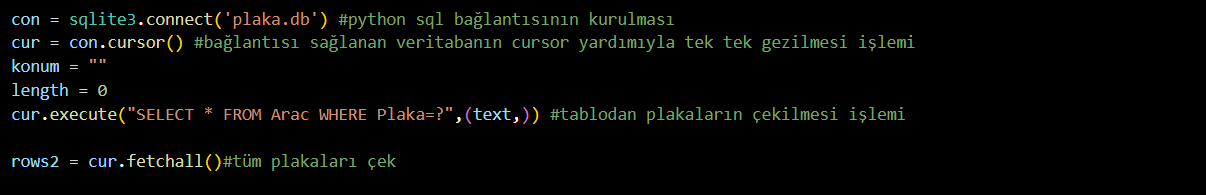
\includegraphics{sql bağlantısı ile python kodları.PNG}
    \caption{Sqlite veritabanına bağlantı sağlama kodları}
    \label{fig:my_label}
\end{figure} \\
\cite{pythonforsqlite}
Bu aşamada ise plakası tanımlanan aracın konumunu kullanıcan girmesini istiyoruz. Eğer otoparkta bu konumda bulunan bir araç yok ise aracın otoparka giriş yapmasını sağlıyoruz. Araç otopark içerisine girdiğinde veritabanında da yer alır. Aracın veritabanında plakası konumu ve giriş zamanı tutulur.

 \begin{figure}
    \centering
    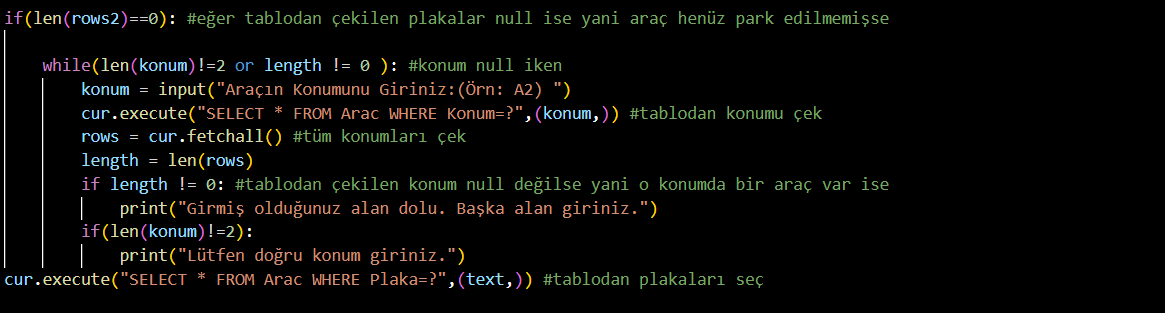
\includegraphics{plakanın konumunun kullanıcıdan alınması.PNG}
    \caption{Plakası tanımlanan aracın konumunun belirlenmesi}
    \label{fig:my_label}
\end{figure} \\
Son kısımda yer alan kodlarımda , aracın plakası daha önce veritabanına kayıtlı ise direkt olarak ücret hesabı ve aracın konumu bildirilip veritabanından aracın kaydının silinmesi işlevi gerçekleştirilirken , plakanın henüz veritabanında kaydı bulunmuyor ise , kaydı oluşturulmaktadır.

\section{PROJEDEN ELDE EDİLEN ÇIKTILARIMIZ}
\subsection{Projenin Çalıştırılması}
 \begin{figure}
    \centering
    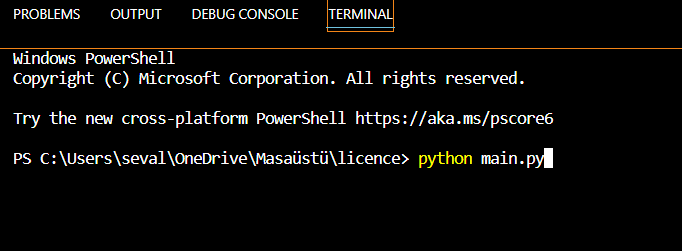
\includegraphics{çalıştırma komutu.PNG}
    \caption{Projenin çalıştırılması için gerekli terminal komutumuz}
    \label{fig:my_label}
\end{figure} \\

\subsection{Kullanıcıdan Resim Inputunun Alınması}
 \begin{figure}
    \centering
    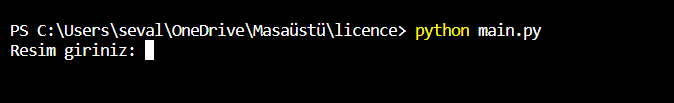
\includegraphics{kullanıcıdan resim girdisi alma.PNG}
    \caption{Kullanıcıdan istenen resim inputu }
    \label{fig:my_label}
\end{figure} \\
\subsection{Kullanıcıdan Alınan Resim Inputuna Göre Plaka Tanımlamasının Yapılması}
Bu kısımda kullanıcın girdiği resim inputu içerisinde bulunan araç resmindeki plaka tanımlanır .
 \begin{figure}
    \centering
    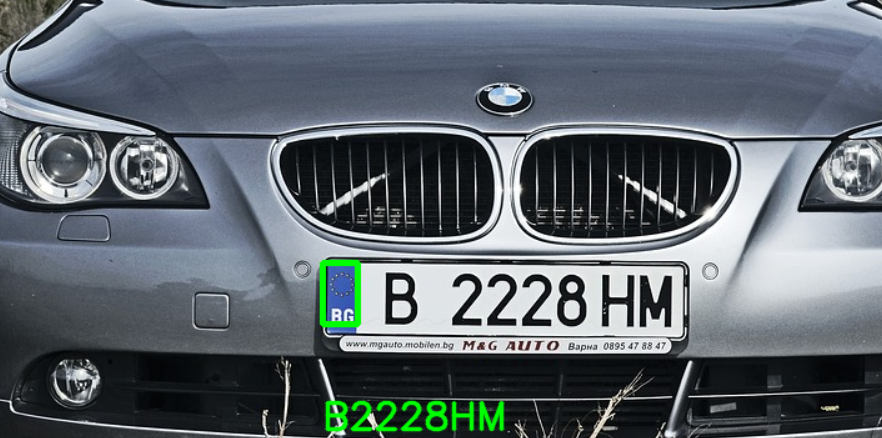
\includegraphics{plaka tanındı.PNG}
    \caption{Kullanıcıdan istenen resim bilgisine göre plakanın işlenmesi }
    \label{fig:my_label}
\end{figure} \\

\subsection{Kullanıcıdan Konum Bilgisinin Alınması}
Bu kısımda hali hazırda tanımlanan plakaya bağlı aracın otoparkın hangi konumunda park edileceği bilgisi kullanıcıdan alınır. \\
Konum bilgisi yalnızca iki haneli olmak zorundadır.\\
Kullanıcının aracı bırakmak istediği konumda bir araç zaten bulunuyor ise kullanıcı başka bir konum girmek zorundadır.\\
 \begin{figure}
    \centering
    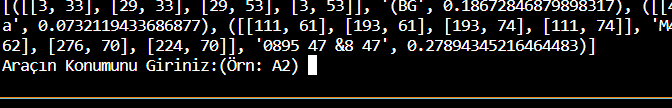
\includegraphics{konum bilgisinin alınması.PNG}
    \caption{Kullanıcıdan tanımlanmış plakaya ait aracın konum bilgisinin alınması }
    \label{fig:my_label}
\end{figure} \\

\subsection{Aracın Otoparktan Ayrılması }
Eğer tanımlanmış plaka öncesinde veritabanında bulunuyor ise biz programı çalıştırdığımızda kullanıcı yine aynı aracın resim bilgisini girdiği zaman plaka ikinci kez veritabanına kaydedilmez. \\
Bu demektir ki araç artık otoparktan ayrılmak istiyor. Böylelikle veritabanından bu plakaya ait bilgilerin kayıtları temizlenir ve otopark ücreti ile aracın konum bilgisi kullanıcıya döndürülür.

 \begin{figure}
    \centering
    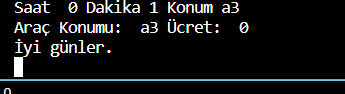
\includegraphics{aracın otoparktan çıkışı.PNG}
    \caption{Aracın otoparktan ayrılması }
    \label{fig:my_label}
\end{figure} \\